% Options for packages loaded elsewhere
\PassOptionsToPackage{unicode}{hyperref}
\PassOptionsToPackage{hyphens}{url}
%
\documentclass[
  letterpaper,
]{book}

\usepackage{amsmath,amssymb}
\usepackage{iftex}
\ifPDFTeX
  \usepackage[T1]{fontenc}
  \usepackage[utf8]{inputenc}
  \usepackage{textcomp} % provide euro and other symbols
\else % if luatex or xetex
  \usepackage{unicode-math}
  \defaultfontfeatures{Scale=MatchLowercase}
  \defaultfontfeatures[\rmfamily]{Ligatures=TeX,Scale=1}
\fi
\usepackage{lmodern}
\ifPDFTeX\else  
    % xetex/luatex font selection
\fi
% Use upquote if available, for straight quotes in verbatim environments
\IfFileExists{upquote.sty}{\usepackage{upquote}}{}
\IfFileExists{microtype.sty}{% use microtype if available
  \usepackage[]{microtype}
  \UseMicrotypeSet[protrusion]{basicmath} % disable protrusion for tt fonts
}{}
\makeatletter
\@ifundefined{KOMAClassName}{% if non-KOMA class
  \IfFileExists{parskip.sty}{%
    \usepackage{parskip}
  }{% else
    \setlength{\parindent}{0pt}
    \setlength{\parskip}{6pt plus 2pt minus 1pt}}
}{% if KOMA class
  \KOMAoptions{parskip=half}}
\makeatother
\usepackage{xcolor}
\setlength{\emergencystretch}{3em} % prevent overfull lines
\setcounter{secnumdepth}{5}
% Make \paragraph and \subparagraph free-standing
\makeatletter
\ifx\paragraph\undefined\else
  \let\oldparagraph\paragraph
  \renewcommand{\paragraph}{
    \@ifstar
      \xxxParagraphStar
      \xxxParagraphNoStar
  }
  \newcommand{\xxxParagraphStar}[1]{\oldparagraph*{#1}\mbox{}}
  \newcommand{\xxxParagraphNoStar}[1]{\oldparagraph{#1}\mbox{}}
\fi
\ifx\subparagraph\undefined\else
  \let\oldsubparagraph\subparagraph
  \renewcommand{\subparagraph}{
    \@ifstar
      \xxxSubParagraphStar
      \xxxSubParagraphNoStar
  }
  \newcommand{\xxxSubParagraphStar}[1]{\oldsubparagraph*{#1}\mbox{}}
  \newcommand{\xxxSubParagraphNoStar}[1]{\oldsubparagraph{#1}\mbox{}}
\fi
\makeatother

\usepackage{color}
\usepackage{fancyvrb}
\newcommand{\VerbBar}{|}
\newcommand{\VERB}{\Verb[commandchars=\\\{\}]}
\DefineVerbatimEnvironment{Highlighting}{Verbatim}{commandchars=\\\{\}}
% Add ',fontsize=\small' for more characters per line
\usepackage{framed}
\definecolor{shadecolor}{RGB}{241,243,245}
\newenvironment{Shaded}{\begin{snugshade}}{\end{snugshade}}
\newcommand{\AlertTok}[1]{\textcolor[rgb]{0.68,0.00,0.00}{#1}}
\newcommand{\AnnotationTok}[1]{\textcolor[rgb]{0.37,0.37,0.37}{#1}}
\newcommand{\AttributeTok}[1]{\textcolor[rgb]{0.40,0.45,0.13}{#1}}
\newcommand{\BaseNTok}[1]{\textcolor[rgb]{0.68,0.00,0.00}{#1}}
\newcommand{\BuiltInTok}[1]{\textcolor[rgb]{0.00,0.23,0.31}{#1}}
\newcommand{\CharTok}[1]{\textcolor[rgb]{0.13,0.47,0.30}{#1}}
\newcommand{\CommentTok}[1]{\textcolor[rgb]{0.37,0.37,0.37}{#1}}
\newcommand{\CommentVarTok}[1]{\textcolor[rgb]{0.37,0.37,0.37}{\textit{#1}}}
\newcommand{\ConstantTok}[1]{\textcolor[rgb]{0.56,0.35,0.01}{#1}}
\newcommand{\ControlFlowTok}[1]{\textcolor[rgb]{0.00,0.23,0.31}{\textbf{#1}}}
\newcommand{\DataTypeTok}[1]{\textcolor[rgb]{0.68,0.00,0.00}{#1}}
\newcommand{\DecValTok}[1]{\textcolor[rgb]{0.68,0.00,0.00}{#1}}
\newcommand{\DocumentationTok}[1]{\textcolor[rgb]{0.37,0.37,0.37}{\textit{#1}}}
\newcommand{\ErrorTok}[1]{\textcolor[rgb]{0.68,0.00,0.00}{#1}}
\newcommand{\ExtensionTok}[1]{\textcolor[rgb]{0.00,0.23,0.31}{#1}}
\newcommand{\FloatTok}[1]{\textcolor[rgb]{0.68,0.00,0.00}{#1}}
\newcommand{\FunctionTok}[1]{\textcolor[rgb]{0.28,0.35,0.67}{#1}}
\newcommand{\ImportTok}[1]{\textcolor[rgb]{0.00,0.46,0.62}{#1}}
\newcommand{\InformationTok}[1]{\textcolor[rgb]{0.37,0.37,0.37}{#1}}
\newcommand{\KeywordTok}[1]{\textcolor[rgb]{0.00,0.23,0.31}{\textbf{#1}}}
\newcommand{\NormalTok}[1]{\textcolor[rgb]{0.00,0.23,0.31}{#1}}
\newcommand{\OperatorTok}[1]{\textcolor[rgb]{0.37,0.37,0.37}{#1}}
\newcommand{\OtherTok}[1]{\textcolor[rgb]{0.00,0.23,0.31}{#1}}
\newcommand{\PreprocessorTok}[1]{\textcolor[rgb]{0.68,0.00,0.00}{#1}}
\newcommand{\RegionMarkerTok}[1]{\textcolor[rgb]{0.00,0.23,0.31}{#1}}
\newcommand{\SpecialCharTok}[1]{\textcolor[rgb]{0.37,0.37,0.37}{#1}}
\newcommand{\SpecialStringTok}[1]{\textcolor[rgb]{0.13,0.47,0.30}{#1}}
\newcommand{\StringTok}[1]{\textcolor[rgb]{0.13,0.47,0.30}{#1}}
\newcommand{\VariableTok}[1]{\textcolor[rgb]{0.07,0.07,0.07}{#1}}
\newcommand{\VerbatimStringTok}[1]{\textcolor[rgb]{0.13,0.47,0.30}{#1}}
\newcommand{\WarningTok}[1]{\textcolor[rgb]{0.37,0.37,0.37}{\textit{#1}}}

\providecommand{\tightlist}{%
  \setlength{\itemsep}{0pt}\setlength{\parskip}{0pt}}\usepackage{longtable,booktabs,array}
\usepackage{calc} % for calculating minipage widths
% Correct order of tables after \paragraph or \subparagraph
\usepackage{etoolbox}
\makeatletter
\patchcmd\longtable{\par}{\if@noskipsec\mbox{}\fi\par}{}{}
\makeatother
% Allow footnotes in longtable head/foot
\IfFileExists{footnotehyper.sty}{\usepackage{footnotehyper}}{\usepackage{footnote}}
\makesavenoteenv{longtable}
\usepackage{graphicx}
\makeatletter
\def\maxwidth{\ifdim\Gin@nat@width>\linewidth\linewidth\else\Gin@nat@width\fi}
\def\maxheight{\ifdim\Gin@nat@height>\textheight\textheight\else\Gin@nat@height\fi}
\makeatother
% Scale images if necessary, so that they will not overflow the page
% margins by default, and it is still possible to overwrite the defaults
% using explicit options in \includegraphics[width, height, ...]{}
\setkeys{Gin}{width=\maxwidth,height=\maxheight,keepaspectratio}
% Set default figure placement to htbp
\makeatletter
\def\fps@figure{htbp}
\makeatother

\makeatletter
\@ifpackageloaded{bookmark}{}{\usepackage{bookmark}}
\makeatother
\makeatletter
\@ifpackageloaded{caption}{}{\usepackage{caption}}
\AtBeginDocument{%
\ifdefined\contentsname
  \renewcommand*\contentsname{Table of contents}
\else
  \newcommand\contentsname{Table of contents}
\fi
\ifdefined\listfigurename
  \renewcommand*\listfigurename{List of Figures}
\else
  \newcommand\listfigurename{List of Figures}
\fi
\ifdefined\listtablename
  \renewcommand*\listtablename{List of Tables}
\else
  \newcommand\listtablename{List of Tables}
\fi
\ifdefined\figurename
  \renewcommand*\figurename{Figure}
\else
  \newcommand\figurename{Figure}
\fi
\ifdefined\tablename
  \renewcommand*\tablename{Table}
\else
  \newcommand\tablename{Table}
\fi
}
\@ifpackageloaded{float}{}{\usepackage{float}}
\floatstyle{ruled}
\@ifundefined{c@chapter}{\newfloat{codelisting}{h}{lop}}{\newfloat{codelisting}{h}{lop}[chapter]}
\floatname{codelisting}{Listing}
\newcommand*\listoflistings{\listof{codelisting}{List of Listings}}
\makeatother
\makeatletter
\makeatother
\makeatletter
\@ifpackageloaded{caption}{}{\usepackage{caption}}
\@ifpackageloaded{subcaption}{}{\usepackage{subcaption}}
\makeatother

\ifLuaTeX
  \usepackage{selnolig}  % disable illegal ligatures
\fi
\usepackage{bookmark}

\IfFileExists{xurl.sty}{\usepackage{xurl}}{} % add URL line breaks if available
\urlstyle{same} % disable monospaced font for URLs
\hypersetup{
  pdftitle={Weikersheim, Residenzschloss},
  pdfauthor={Team Redaktion},
  hidelinks,
  pdfcreator={LaTeX via pandoc}}


\title{Weikersheim, Residenzschloss}
\author{Team Redaktion}
\date{2024-03-22}

\begin{document}
\frontmatter
\maketitle

\renewcommand*\contentsname{Table of contents}
{
\setcounter{tocdepth}{2}
\tableofcontents
}

\mainmatter
\bookmarksetup{startatroot}

\chapter{Katalog zur Ausstellung: Der Große Saal
(Rittersaal)}\label{katalog-zur-ausstellung-der-grouxdfe-saal-rittersaal}

Ein Katalog mit Kunstwerken aus der CbDD-Sammlung. Textteil:
\href{https://www.deckenmalerei.eu/6e73f774-4b7f-4e37-937b-e11cc35c5bc8}{6e73f774-4b7f-4e37-937b-e11cc35c5bc8}

Der Große Saal (Rittersaal) {[}Raum{]}

This work is licensed under a Creative Commons
Attribution-NonCommercial-NoDerivs 4.0 International License.

\bookmarksetup{startatroot}

\chapter{Die Saaldecke der Renaissance von Balthasar
Katzenberger}\label{die-saaldecke-der-renaissance-von-balthasar-katzenberger}

\begin{Shaded}
\begin{Highlighting}[]
\ImportTok{from}\NormalTok{ datetime }\ImportTok{import}\NormalTok{ datetime}
\ImportTok{import}\NormalTok{ sys}
\ImportTok{import}\NormalTok{ time}
\ImportTok{from}\NormalTok{ SPARQLWrapper }\ImportTok{import}\NormalTok{ SPARQLWrapper, JSON}
\ImportTok{import}\NormalTok{ requests}
\ImportTok{from}\NormalTok{ PIL }\ImportTok{import}\NormalTok{ Image}
\ImportTok{import}\NormalTok{ html}

\NormalTok{endpoint\_url }\OperatorTok{=} \StringTok{"https://computational{-}publishing{-}service.wikibase.cloud/query/sparql"}

\NormalTok{query\_txt }\OperatorTok{=} \StringTok{"""PREFIX cps: \textless{}https://computational{-}publishing{-}service.wikibase.cloud/entity/\textgreater{}}
\StringTok{PREFIX cpss: \textless{}https://computational{-}publishing{-}service.wikibase.cloud/entity/statement/\textgreater{}}
\StringTok{PREFIX cpsv: \textless{}https://computational{-}publishing{-}service.wikibase.cloud/value/\textgreater{}}
\StringTok{PREFIX cpspt: \textless{}https://computational{-}publishing{-}service.wikibase.cloud/prop/direct/\textgreater{}}
\StringTok{PREFIX cpsp: \textless{}https://computational{-}publishing{-}service.wikibase.cloud/prop/\textgreater{}}
\StringTok{PREFIX cpsps: \textless{}https://computational{-}publishing{-}service.wikibase.cloud/prop/statement/\textgreater{}}
\StringTok{PREFIX cpspq: \textless{}https://computational{-}publishing{-}service.wikibase.cloud/prop/qualifier/\textgreater{}}


\StringTok{SELECT ?textItem ?kuratorLabel ?textUrl}
\StringTok{WHERE}
\StringTok{\{}
\StringTok{  \textless{}placeholder\textgreater{}}
\StringTok{  ?textItem cpsp:P46 ?kuratorStatement. }
\StringTok{  ?kuratorStatement cpsps:P46 ?kuratorItem. }
\StringTok{  ?kuratorItem rdfs:label ?kuratorLabel.}
\StringTok{  ?textItem cpsp:P57 ?urlstatement. }
\StringTok{  ?urlstatement cpsps:P57 ?textUrl. }
\StringTok{\}"""}

\NormalTok{query\_img }\OperatorTok{=}\StringTok{"""PREFIX cps: \textless{}https://computational{-}publishing{-}service.wikibase.cloud/entity/\textgreater{}}
\StringTok{PREFIX cpss: \textless{}https://computational{-}publishing{-}service.wikibase.cloud/entity/statement/\textgreater{}}
\StringTok{PREFIX cpsv: \textless{}https://computational{-}publishing{-}service.wikibase.cloud/value/\textgreater{}}
\StringTok{PREFIX cpspt: \textless{}https://computational{-}publishing{-}service.wikibase.cloud/prop/direct/\textgreater{}}
\StringTok{PREFIX cpsp: \textless{}https://computational{-}publishing{-}service.wikibase.cloud/prop/\textgreater{}}
\StringTok{PREFIX cpsps: \textless{}https://computational{-}publishing{-}service.wikibase.cloud/prop/statement/\textgreater{}}
\StringTok{PREFIX cpspq: \textless{}https://computational{-}publishing{-}service.wikibase.cloud/prop/qualifier/\textgreater{}}

\StringTok{SELECT DISTINCT ?itemLabel ?itemDescr ?imgItem ?imgUrl ?publishDate}
\StringTok{WHERE}
\StringTok{\{}
\StringTok{  ?imgItem cpsp:P107 ?urlStatement. }
\StringTok{  ?urlStatement cpsps:P107 ?imgUrl. }
\StringTok{  ?imgItem cpsp:P60 ?dateStatement. }
\StringTok{  ?dateStatement cpsps:P60 ?publishDate. }
\StringTok{  ?imgItem cpsp:P6 ?partOfStatement.}
\StringTok{  ?partOfStatement cpsps:P6 ?partOfItem.}
\StringTok{  \textless{}placeholder\textgreater{} }

\StringTok{  FILTER (datatype(?publishDate) = xsd:edtf)}
\StringTok{  }
\StringTok{  SERVICE wikibase:label \{}
\StringTok{      bd:serviceParam wikibase:language "en,de".}
\StringTok{      ?imgItem rdfs:label ?itemLabel.}
\StringTok{      ?imgItem schema:description ?itemDescr.}
\StringTok{    \}}
\StringTok{\}"""}
\NormalTok{query\_graph }\OperatorTok{=} \StringTok{"""PREFIX cps: \textless{}https://computational{-}publishing{-}service.wikibase.cloud/entity/\textgreater{}}
\StringTok{PREFIX cpss: \textless{}https://computational{-}publishing{-}service.wikibase.cloud/entity/statement/\textgreater{}}
\StringTok{PREFIX cpsv: \textless{}https://computational{-}publishing{-}service.wikibase.cloud/value/\textgreater{}}
\StringTok{PREFIX cpspt: \textless{}https://computational{-}publishing{-}service.wikibase.cloud/prop/direct/\textgreater{}}
\StringTok{PREFIX cpsp: \textless{}https://computational{-}publishing{-}service.wikibase.cloud/prop/\textgreater{}}
\StringTok{PREFIX cpsps: \textless{}https://computational{-}publishing{-}service.wikibase.cloud/prop/statement/\textgreater{}}
\StringTok{PREFIX cpspq: \textless{}https://computational{-}publishing{-}service.wikibase.cloud/prop/qualifier/\textgreater{}}

\StringTok{SELECT ?x ?y}
\StringTok{WHERE}
\StringTok{\{}
\StringTok{  ?a cpsp:P2 ?c.}
\StringTok{  ?c cpsps:P2 ?d.}
\StringTok{  ?a rdfs:label ?x.}
\StringTok{  ?d rdfs:label ?y.}

\StringTok{\}LIMIT 1"""}

\NormalTok{query\_graph2 }\OperatorTok{=} \StringTok{"""}
\StringTok{SELECT ?a ?b ?c}
\StringTok{WHERE}
\StringTok{\{}
\StringTok{  ?a rdfs:label ?c}
\StringTok{\}LIMIT 100"""}


\KeywordTok{def}\NormalTok{ run\_query(endpoint\_url, query):}
\NormalTok{    user\_agent }\OperatorTok{=} \StringTok{"WDQS{-}example Python/}\SpecialCharTok{\%s}\StringTok{.}\SpecialCharTok{\%s}\StringTok{"} \OperatorTok{\%}\NormalTok{ (sys.version\_info[}\DecValTok{0}\NormalTok{], sys.version\_info[}\DecValTok{1}\NormalTok{])}
    \CommentTok{\# }\AlertTok{TODO}\CommentTok{ adjust user agent; see https://w.wiki/CX6}
\NormalTok{    sparql }\OperatorTok{=}\NormalTok{ SPARQLWrapper(endpoint\_url, agent}\OperatorTok{=}\NormalTok{user\_agent)}
\NormalTok{    sparql.setQuery(query)}
\NormalTok{    sparql.setMethod(}\StringTok{"POST"}\NormalTok{) }\CommentTok{\#this NEEDS to be added to get results (not included in the wikibase python example code)}
\NormalTok{    sparql.setReturnFormat(JSON)}
    \ControlFlowTok{return}\NormalTok{ sparql.query().convert()}

\KeywordTok{def}\NormalTok{ get\_text(textitem\_id):}
\NormalTok{    q }\OperatorTok{=} \StringTok{""}
    \ControlFlowTok{if}\NormalTok{ textitem\_id:}
\NormalTok{        q }\OperatorTok{=}\NormalTok{ query\_txt.replace(}\StringTok{"\textless{}placeholder\textgreater{}"}\NormalTok{, }\StringTok{"cps:"}\OperatorTok{+}\NormalTok{textitem\_id}\OperatorTok{+}\StringTok{" cpsp:P46 ?kuratorStatement."}\NormalTok{)}
    \ControlFlowTok{else}\NormalTok{:}
\NormalTok{        q }\OperatorTok{=}\NormalTok{ query\_txt.replace(}\StringTok{"\textless{}placeholder\textgreater{}"}\NormalTok{,}\StringTok{""}\NormalTok{)}

\NormalTok{    results\_txt }\OperatorTok{=}\NormalTok{ run\_query(endpoint\_url, q)}
    \ControlFlowTok{for}\NormalTok{ item }\KeywordTok{in}\NormalTok{ results\_txt[}\StringTok{"results"}\NormalTok{][}\StringTok{"bindings"}\NormalTok{]:}
        \CommentTok{\# print(item)}
        \BuiltInTok{print}\NormalTok{(}\StringTok{\textquotesingle{}Wikibase link: \textquotesingle{}} \OperatorTok{+} \StringTok{\textquotesingle{}[\textquotesingle{}} \OperatorTok{+}\NormalTok{ item[}\StringTok{\textquotesingle{}textItem\textquotesingle{}}\NormalTok{][}\StringTok{\textquotesingle{}value\textquotesingle{}}\NormalTok{] }\OperatorTok{+} \StringTok{\textquotesingle{}]\textquotesingle{}} \OperatorTok{+} \StringTok{\textquotesingle{}(\textquotesingle{}} \OperatorTok{+}\NormalTok{ item[}\StringTok{\textquotesingle{}textItem\textquotesingle{}}\NormalTok{][}\StringTok{\textquotesingle{}value\textquotesingle{}}\NormalTok{] }\OperatorTok{+} \StringTok{\textquotesingle{})\textquotesingle{}} \OperatorTok{+} \StringTok{\textquotesingle{}}\CharTok{\textbackslash{}n}\StringTok{\textquotesingle{}}\NormalTok{)}
        \BuiltInTok{print}\NormalTok{(}\StringTok{\textquotesingle{}Kurator: \textquotesingle{}} \OperatorTok{+}\NormalTok{ item[}\StringTok{\textquotesingle{}kuratorLabel\textquotesingle{}}\NormalTok{][}\StringTok{\textquotesingle{}value\textquotesingle{}}\NormalTok{] }\OperatorTok{+} \StringTok{\textquotesingle{}}\CharTok{\textbackslash{}n}\StringTok{\textquotesingle{}}\NormalTok{)}
\NormalTok{        headers }\OperatorTok{=}\NormalTok{ \{}\StringTok{\textquotesingle{}User{-}Agent\textquotesingle{}}\NormalTok{: }\StringTok{\textquotesingle{}Ex\_Books\_conference\_bot/0.0 (https://github.com/SimonXIX/Experimental\_Books\_workshop; ad7588@coventry.ac.uk)\textquotesingle{}}\NormalTok{\}}
\NormalTok{        r }\OperatorTok{=}\NormalTok{ requests.get(item[}\StringTok{\textquotesingle{}textUrl\textquotesingle{}}\NormalTok{][}\StringTok{\textquotesingle{}value\textquotesingle{}}\NormalTok{], headers}\OperatorTok{=}\NormalTok{headers, stream}\OperatorTok{=}\VariableTok{True}\NormalTok{)}
\NormalTok{        text }\OperatorTok{=} \BuiltInTok{str}\NormalTok{(r.content)}
\NormalTok{        text }\OperatorTok{=}\NormalTok{ text.replace(}\StringTok{"ä"}\NormalTok{,}\StringTok{"\&auml;"}\NormalTok{)}
\NormalTok{        text }\OperatorTok{=}\NormalTok{ text.replace(}\StringTok{"Ä"}\NormalTok{,}\StringTok{"\&Auml;"}\NormalTok{)}
\NormalTok{        text }\OperatorTok{=}\NormalTok{ text.replace(}\StringTok{"ö"}\NormalTok{,}\StringTok{"\&ouml;"}\NormalTok{)}
\NormalTok{        text }\OperatorTok{=}\NormalTok{ text.replace(}\StringTok{"Ö"}\NormalTok{,}\StringTok{"\&Ouml;"}\NormalTok{)}
\NormalTok{        text }\OperatorTok{=}\NormalTok{ text.replace(}\StringTok{"ü"}\NormalTok{,}\StringTok{"\&uuml;"}\NormalTok{)}
\NormalTok{        text }\OperatorTok{=}\NormalTok{ text.replace(}\StringTok{"Ü"}\NormalTok{,}\StringTok{"\&Uuml;"}\NormalTok{)}
\NormalTok{        text }\OperatorTok{=}\NormalTok{ text.replace(}\StringTok{"ß"}\NormalTok{,}\StringTok{"\&szlig;"}\NormalTok{)}
\NormalTok{        text }\OperatorTok{=}\NormalTok{ text.replace(}\StringTok{\textquotesingle{}}\CharTok{\textbackslash{}\textbackslash{}}\StringTok{n\textquotesingle{}}\NormalTok{,}\StringTok{"\textless{}br\textgreater{}"}\NormalTok{)}
\NormalTok{        text }\OperatorTok{=} \BuiltInTok{str}\NormalTok{(text)}
\NormalTok{        text }\OperatorTok{=}\NormalTok{ text.removeprefix(}\StringTok{"b\textquotesingle{}\textless{}!DOCTYPE html\textgreater{}"}\NormalTok{).removesuffix(}\StringTok{"\textquotesingle{}"}\NormalTok{)}
        \BuiltInTok{print}\NormalTok{(text)}

\KeywordTok{def}\NormalTok{ get\_delay(date):}
    \ControlFlowTok{try}\NormalTok{:}
\NormalTok{        date }\OperatorTok{=}\NormalTok{ datetime.datetime.strptime(date, }\StringTok{\textquotesingle{}\%a, }\SpecialCharTok{\%d}\StringTok{ \%b \%Y \%H:\%M:\%S GMT\textquotesingle{}}\NormalTok{)}
\NormalTok{        timeout }\OperatorTok{=} \BuiltInTok{int}\NormalTok{((date }\OperatorTok{{-}}\NormalTok{ datetime.datetime.now()).total\_seconds())}
    \ControlFlowTok{except} \PreprocessorTok{ValueError}\NormalTok{:}
\NormalTok{        timeout }\OperatorTok{=} \BuiltInTok{int}\NormalTok{(date)}
    \ControlFlowTok{return}\NormalTok{ timeout}

\KeywordTok{def}\NormalTok{ fetch\_image\_by\_url(url, headers):}
\NormalTok{    r }\OperatorTok{=}\NormalTok{ requests.get(url, headers}\OperatorTok{=}\NormalTok{headers, stream}\OperatorTok{=}\VariableTok{True}\NormalTok{)}
    \ControlFlowTok{if}\NormalTok{ r.status\_code }\OperatorTok{==} \DecValTok{200}\NormalTok{:}
\NormalTok{        im }\OperatorTok{=}\NormalTok{ Image.}\BuiltInTok{open}\NormalTok{(r.raw)}
        \ControlFlowTok{return}\NormalTok{ im}
    \ControlFlowTok{if}\NormalTok{ r.status\_code }\OperatorTok{==} \DecValTok{500}\NormalTok{:}
        \ControlFlowTok{return} \VariableTok{None}
    \ControlFlowTok{if}\NormalTok{ r.status\_code }\OperatorTok{==} \DecValTok{403}\NormalTok{:}
        \ControlFlowTok{return} \VariableTok{None}
    \ControlFlowTok{if}\NormalTok{ r.status\_code }\OperatorTok{==} \DecValTok{429}\NormalTok{:}
\NormalTok{        timeout }\OperatorTok{=}\NormalTok{ get\_delay(r.headers[}\StringTok{\textquotesingle{}retry{-}after\textquotesingle{}}\NormalTok{])}
        \BuiltInTok{print}\NormalTok{(}\StringTok{\textquotesingle{}Timeout }\SpecialCharTok{\{\}}\StringTok{ m }\SpecialCharTok{\{\}}\StringTok{ s\textquotesingle{}}\NormalTok{.}\BuiltInTok{format}\NormalTok{(timeout }\OperatorTok{//} \DecValTok{60}\NormalTok{, timeout }\OperatorTok{\%} \DecValTok{60}\NormalTok{))}
\NormalTok{        time.sleep(timeout)}
\NormalTok{        fetch\_image\_by\_url(url, headers)}

\KeywordTok{def}\NormalTok{ get\_img(partOfItem\_id):}
\NormalTok{    q }\OperatorTok{=} \StringTok{""}
    \ControlFlowTok{if}\NormalTok{ partOfItem\_id:}
\NormalTok{        q }\OperatorTok{=}\NormalTok{ query\_img.replace(}\StringTok{"\textless{}placeholder\textgreater{}"}\NormalTok{, }\StringTok{"?partOfStatement cpsps:P6 cps:"}\OperatorTok{+}\NormalTok{partOfItem\_id}\OperatorTok{+}\StringTok{"."}\NormalTok{)}
    \ControlFlowTok{else}\NormalTok{:}
\NormalTok{        q }\OperatorTok{=}\NormalTok{ query\_img.replace(}\StringTok{"\textless{}placeholder\textgreater{}"}\NormalTok{,}\StringTok{""}\NormalTok{)}
\NormalTok{    results\_img }\OperatorTok{=}\NormalTok{ run\_query(endpoint\_url, q)}
    \ControlFlowTok{for}\NormalTok{ item }\KeywordTok{in}\NormalTok{ results\_img[}\StringTok{"results"}\NormalTok{][}\StringTok{"bindings"}\NormalTok{]:    }
      \CommentTok{\#print(item)}
      \BuiltInTok{print}\NormalTok{(}\StringTok{\textquotesingle{}Wikibase link: \textquotesingle{}} \OperatorTok{+} \StringTok{\textquotesingle{}[\textquotesingle{}} \OperatorTok{+}\NormalTok{ item[}\StringTok{\textquotesingle{}imgItem\textquotesingle{}}\NormalTok{][}\StringTok{\textquotesingle{}value\textquotesingle{}}\NormalTok{] }\OperatorTok{+} \StringTok{\textquotesingle{}]\textquotesingle{}} \OperatorTok{+} \StringTok{\textquotesingle{}(\textquotesingle{}} \OperatorTok{+}\NormalTok{ item[}\StringTok{\textquotesingle{}imgItem\textquotesingle{}}\NormalTok{][}\StringTok{\textquotesingle{}value\textquotesingle{}}\NormalTok{] }\OperatorTok{+} \StringTok{\textquotesingle{})\textquotesingle{}} \OperatorTok{+} \StringTok{\textquotesingle{}}\CharTok{\textbackslash{}n}\StringTok{\textquotesingle{}}\NormalTok{)}
      \BuiltInTok{print}\NormalTok{(}\StringTok{\textquotesingle{}Title: \textquotesingle{}} \OperatorTok{+}\NormalTok{ item[}\StringTok{\textquotesingle{}itemLabel\textquotesingle{}}\NormalTok{][}\StringTok{\textquotesingle{}value\textquotesingle{}}\NormalTok{] }\OperatorTok{+} \StringTok{\textquotesingle{}}\CharTok{\textbackslash{}n}\StringTok{\textquotesingle{}}\NormalTok{)}
      \BuiltInTok{print}\NormalTok{(}\StringTok{\textquotesingle{}Year: \textquotesingle{}} \OperatorTok{+}\NormalTok{ item[}\StringTok{\textquotesingle{}publishDate\textquotesingle{}}\NormalTok{][}\StringTok{\textquotesingle{}value\textquotesingle{}}\NormalTok{] }\OperatorTok{+} \StringTok{\textquotesingle{}}\CharTok{\textbackslash{}n}\StringTok{\textquotesingle{}}\NormalTok{)}
      \BuiltInTok{print}\NormalTok{(}\StringTok{\textquotesingle{}Description: \textquotesingle{}} \OperatorTok{+}\NormalTok{ html.unescape(item[}\StringTok{\textquotesingle{}itemDescr\textquotesingle{}}\NormalTok{][}\StringTok{\textquotesingle{}value\textquotesingle{}}\NormalTok{]) }\OperatorTok{+} \StringTok{\textquotesingle{}}\CharTok{\textbackslash{}n}\StringTok{\textquotesingle{}}\NormalTok{)}

      \CommentTok{\# get image from image URL and display resized version}
\NormalTok{      image\_url}\OperatorTok{=}\NormalTok{item[}\StringTok{\textquotesingle{}imgUrl\textquotesingle{}}\NormalTok{][}\StringTok{\textquotesingle{}value\textquotesingle{}}\NormalTok{]}
\NormalTok{      headers }\OperatorTok{=}\NormalTok{ \{}\StringTok{\textquotesingle{}User{-}Agent\textquotesingle{}}\NormalTok{: }\StringTok{\textquotesingle{}Ex\_Books\_conference\_bot/0.0 (https://github.com/SimonXIX/Experimental\_Books\_workshop; ad7588@coventry.ac.uk)\textquotesingle{}}\NormalTok{\}}
\NormalTok{      im }\OperatorTok{=}\NormalTok{ fetch\_image\_by\_url(image\_url, headers)}
\NormalTok{      im.thumbnail((}\DecValTok{500}\NormalTok{, }\DecValTok{500}\NormalTok{), Image.Resampling.LANCZOS)}
\NormalTok{      display(im)}
      \BuiltInTok{print}\NormalTok{(}\StringTok{\textquotesingle{}}\CharTok{\textbackslash{}n\textbackslash{}n}\StringTok{\textquotesingle{}}\NormalTok{)}

\KeywordTok{def}\NormalTok{ get\_graph():}
    \ImportTok{import}\NormalTok{ VizKG.visualize }\ImportTok{as}\NormalTok{ vkg}
\NormalTok{    results\_graph1 }\OperatorTok{=}\NormalTok{ run\_query(endpoint\_url, query\_graph)}
    \CommentTok{\#print(results\_graph1)}
    \CommentTok{\#print(\textquotesingle{}{-}{-}{-}\textquotesingle{})}
\NormalTok{    results\_graph2 }\OperatorTok{=}\NormalTok{ run\_query(endpoint\_url, query\_graph2)}
    \CommentTok{\#print(results\_graph2)}

\NormalTok{    chart }\OperatorTok{=}\NormalTok{ vkg(sparql\_query}\OperatorTok{=}\NormalTok{query\_graph2, sparql\_service\_url}\OperatorTok{=}\NormalTok{endpoint\_url, chart}\OperatorTok{=}\StringTok{\textquotesingle{}wordcloud\textquotesingle{}}\NormalTok{)}
\NormalTok{    chart.plot()}
\end{Highlighting}
\end{Shaded}

\textbf{How to use your own text for processing}

\begin{enumerate}
\def\labelenumi{\arabic{enumi}.}
\tightlist
\item
  Add a new Text item to the wikibase.
  \href{https://computational-publishing-service.wikibase.cloud/wiki/Special:NewItem}{link
  to wikibase new item} the item should contain the following
  statements:
\end{enumerate}

\begin{itemize}
\tightlist
\item
  P57 (external link): link to the html file containing the new text
\item
  P46 (kurator): Item of the curator. you may use an existing item like
  Q210 (Ulrike seeger) for test purposes
\item
  P53 (license): Item of a license for the text. e.g Q203 (CC BY-NC-ND
  4.0 DEED )
\item
  P6 (is part of): set value to Q218 (Schlossanlage Weikersheim)
\end{itemize}

\begin{enumerate}
\def\labelenumi{\arabic{enumi}.}
\setcounter{enumi}{1}
\item
  check if your new text item occurs in the list of selected text items:
  \href{https://computational-publishing-service.wikibase.cloud/query/\#PREFIX\%20cps\%3A\%20\%3Chttps\%3A\%2F\%2Fcomputational-publishing-service.wikibase.cloud\%2Fentity\%2F\%3E\%0APREFIX\%20cpss\%3A\%20\%3Chttps\%3A\%2F\%2Fcomputational-publishing-service.wikibase.cloud\%2Fentity\%2Fstatement\%2F\%3E\%0APREFIX\%20cpsv\%3A\%20\%3Chttps\%3A\%2F\%2Fcomputational-publishing-service.wikibase.cloud\%2Fvalue\%2F\%3E\%0APREFIX\%20cpspt\%3A\%20\%3Chttps\%3A\%2F\%2Fcomputational-publishing-service.wikibase.cloud\%2Fprop\%2Fdirect\%2F\%3E\%0APREFIX\%20cpsp\%3A\%20\%3Chttps\%3A\%2F\%2Fcomputational-publishing-service.wikibase.cloud\%2Fprop\%2F\%3E\%0APREFIX\%20cpsps\%3A\%20\%3Chttps\%3A\%2F\%2Fcomputational-publishing-service.wikibase.cloud\%2Fprop\%2Fstatement\%2F\%3E\%0APREFIX\%20cpspq\%3A\%20\%3Chttps\%3A\%2F\%2Fcomputational-publishing-service.wikibase.cloud\%2Fprop\%2Fqualifier\%2F\%3E\%0A\%0ASELECT\%20\%3FtextItem\%20\%3FkuratorLabel\%20\%3FtextUrl\%0AWHERE\%0A\%7B\%0A\%20\%20\%3FtextItem\%20cpsp\%3AP46\%20\%3FkuratorStatement.\%20\%0A\%20\%20\%3FkuratorStatement\%20cpsps\%3AP46\%20\%3FkuratorItem.\%20\%0A\%20\%20\%3FkuratorItem\%20rdfs\%3Alabel\%20\%3FkuratorLabel.\%0A\%20\%20\%3FtextItem\%20cpsp\%3AP57\%20\%3Furlstatement.\%20\%0A\%20\%20\%3Furlstatement\%20cpsps\%3AP57\%20\%3FtextUrl.\%20\%0A\%7D}{Link
  to wikibase query service}
\item
  set parameter of get\_text() to the id of your new text item e.g.:
  get\_text(``Q209'')
\end{enumerate}

\begin{Shaded}
\begin{Highlighting}[]
\NormalTok{get\_text(}\StringTok{"Q229"}\NormalTok{)}
\end{Highlighting}
\end{Shaded}

Wikibase link:
\url{https://computational-publishing-service.wikibase.cloud/entity/Q229}

Kurator: Seeger, Ulrike

b'\textless!DOCTYPE html\textgreater{}

Die Saaldecke der Renaissance von Balthasar Katzenberger

Vertragsbedingungen

Der Vertrag zu den 69 Deckengemälden des Großen Saals zwischen Graf
Wolfgang und Balthasar Katzenberger hat sich erhalten.{[}1{]} Darin
wurde am 22. September 1601 festgelegt, dass der Maler Balthasar
Katzenberger aus Würzburg „Ihren gnaden {[}Graf Wolfgang{]} die deckh im
Neuen Saal mit Wasserfarb auff Tuech von allerlej Jagden, Waydtwerkh und
andern was Ire g. Ime jedesmals fürgeben und beuehlen laßen, aufs
schönst Säuberst, Künstlichstelichen und frech aussehendt mallen soll,
alle Simbs der gannzen Deckh sowoll auch neben herrumb das Simbs alles
mit brauner nus oder sonsten ein Dunckhel holz färb, wie es Iren gnaden
gefellig anstreichen``.{[}2{]}

Graf Wolfgang scheint sowohl das Thema der Jagd vorgegeben als auch die
zugehörigen druckgraphischen Vorlagen zur Verfügung gestellt zu haben.
Den Passus „allerlej Jagden, Waydtwerkh und andern was Ire g. Ime
jedesmals fürgeben und beuehlen laßen`` hat man wahrscheinlich
dahingehend zu deuten, dass der Auftraggeber in absehbarer Zeit noch
weitere Vorlagen liefern könnte. Die zur Anwendung gelangte Technik „mit
Wasserfarb auff Tuech`` scheint nur die zweite Wahl gewesen zu sein. In
den Vertrag wurde der Zusatz aufgenommen, dass, sollte Graf Wolfgang
sich doch noch für Ölfarben entscheiden, er anstatt der vereinbarten 195
Gulden 260 Gulden zu zahlen habe, jeweils zuzüglich der täglichen
Verpflegung:

„Da {[}= Falls{]} es aber Ihren Gnaden gefellig wer solche deckh mit öll
färb zuverferttigen soll Ihme für seine belohnung gegeben werden, Zway
hundert und Sechzig gülden. Die Cost und Suppen wie gemelt``.{[}3{]}

Laut Restaurierungsbericht malte Katzenberger in Leimfarben auf grober,
hellgelb grundierter Leinwand.{[}4{]} Erst Christian Thalwitzer, der die
Gemälde 1710/11 überarbeitete, verstärkte ihre Leuchtkraft mit einer
roten Grundierung und Ölfarben, was ebenfalls die Restaurierung der
Jahre 1982--1989 erbrachte. Eines der quadratischen Gemälde (Q1)
überliefert auf der Rückseite die originale Maltechnik. Katzenberger
hatte das Gemälde angelegt und in der rechten Bildhälfte nahezu
fertiggestellt, als sich für die in der linken Bildhälfte angelegte
Figur eine Änderung ergab. Da Leimfarben schlecht decken, verzichtete er
auf eine Übermalung und drehte die Leinwand kurzerhand um.{[}5{]}

Die Gemälde entstanden in der Werkstatt, wobei für die achteckigen
Gemälde mit einer Höhe von 3,65 Metern ein Gerüst gezimmert werden
musste. Da der Vertrag zu Beginn der dunklen Jahreszeit Ende September
abgeschlossen wurde, legte Graf Wolfgang vorsorglich fest, dass
Katzenberger nur bei Tageslicht malen dürfe: „In Summa solche Deckh wie
gemelt {[}= wie oben vereinbart{]} er selbsten alles bej tag und nit bej
nacht aufs Künstlichst und schönst machen und verferttigen``. Der
Auftraggeber stellte die Leinwand, die Farben, Gold und Steinöl für die
Gesimse. Gemalt hat Katzenberger die Bilder unter Aufsicht des Grafen in
Weikersheim, da sein Lohn neben den 195 Gulden aus morgendlicher und
abendlicher Verpflegung mit Brot und Suppe ohne Fleisch bestand.

Katzenberger benötigte für die Arbeit, die er ganz allein, also ohne
Kompagnon, nur mit Malergehilfen leistete, dreizehn Monate. Die
Fertigstellung quittierte er am 22. November 1602.{[}6{]} In die
zahlreichen Künstlersignaturen von Graf Wolfgangs Renaissanceausstattung
reihte er sich auf dem Achteck-Gemälde Nr. 13 ein, das sich knapp
östlich der Mitte der Decke befindet. Sinnfällig nutzte er das Thema der
Wildkatzenjagd für ein Selbstporträt mit Pinsel, Malstock und Palette.
Rechts unten notierte er in schwarzer Schrift: „Balthasar Katzenberger
vo{[}n{]} Wurtzburg maler hat diese gantze Decken in ⋅ 13 ⋅ monat
alleins gemalet 1602``.{[}7{]} Rechnet man sechs Arbeitstage pro Woche,
so entfallen fünf Tage auf ein Bild, wobei freilich die 12 Blumenbilder
deutlich weniger Zeit in Anspruch nahmen als die 19 großen
Achteckbilder.

Balthasar Katzenberger schuf für Schloss Weikersheim seine
umfangreichsten erhaltenen Werke. Über weitere Anhaltspunkte zu seinem
Oeuvre und seinem Lebensweg unterrichtet der Eintrag im Allgemeinen
Künstlerlexikon.{[}8{]}

\textbf{How to select images for processing}

Images are selected via the sparql query. The method get\_img() is
capable of using a wikibase item id as parameter to select images with
the property P6 (is part of) linking to the given item id.

\begin{enumerate}
\def\labelenumi{\arabic{enumi}.}
\item
  select a valid location id from the query result:
  \href{https://computational-publishing-service.wikibase.cloud/query/\#PREFIX\%20cps\%3A\%20\%3Chttps\%3A\%2F\%2Fcomputational-publishing-service.wikibase.cloud\%2Fentity\%2F\%3E\%0APREFIX\%20cpss\%3A\%20\%3Chttps\%3A\%2F\%2Fcomputational-publishing-service.wikibase.cloud\%2Fentity\%2Fstatement\%2F\%3E\%0APREFIX\%20cpsv\%3A\%20\%3Chttps\%3A\%2F\%2Fcomputational-publishing-service.wikibase.cloud\%2Fvalue\%2F\%3E\%0APREFIX\%20cpspt\%3A\%20\%3Chttps\%3A\%2F\%2Fcomputational-publishing-service.wikibase.cloud\%2Fprop\%2Fdirect\%2F\%3E\%0APREFIX\%20cpsp\%3A\%20\%3Chttps\%3A\%2F\%2Fcomputational-publishing-service.wikibase.cloud\%2Fprop\%2F\%3E\%0APREFIX\%20cpsps\%3A\%20\%3Chttps\%3A\%2F\%2Fcomputational-publishing-service.wikibase.cloud\%2Fprop\%2Fstatement\%2F\%3E\%0APREFIX\%20cpspq\%3A\%20\%3Chttps\%3A\%2F\%2Fcomputational-publishing-service.wikibase.cloud\%2Fprop\%2Fqualifier\%2F\%3E\%0A\%0ASELECT\%20DISTINCT\%20\%3FpartOfItem\%20\%3FpartOfItemLabel\%0AWHERE\%0A\%7B\%0A\%20\%20\%3FimgItem\%20cpsp\%3AP107\%20\%3FurlStatement.\%20\%0A\%20\%20\%3FurlStatement\%20cpsps\%3AP107\%20\%3FimgUrl.\%20\%0A\%20\%20\%3FimgItem\%20cpsp\%3AP60\%20\%3FdateStatement.\%20\%0A\%20\%20\%3FdateStatement\%20cpsps\%3AP60\%20\%3FpublishDate.\%20\%0A\%20\%20\%3FimgItem\%20cpsp\%3AP6\%20\%3FpartOfStatement.\%0A\%20\%20\%3FpartOfStatement\%20cpsps\%3AP6\%20\%3FpartOfItem.\%0A\%20\%20SERVICE\%20wikibase\%3Alabel\%20\%7B\%0A\%20\%20\%20\%20\%20\%20bd\%3AserviceParam\%20wikibase\%3Alanguage\%20\%22de\%2Cen\%22.\%0A\%20\%20\%20\%20\%20\%20\%3FpartOfItem\%20rdfs\%3Alabel\%20\%3FpartOfItemLabel.\%0A\%20\%20\%20\%20\%20\%20\%3FpartOfItem\%20schema\%3Adescription\%20\%3FpartOfItemDescr.\%0A\%20\%20\%20\%20\%7D\%0A\%7D\%20GROUP\%20BY\%20\%3FpartOfItem\%20\%3FpartOfItemLabel}{Link
  to wikibase query service}
\item
  set parameter of get\_img() to the id of your selected location item
  e.g.: get\_img(``Q217'')
\end{enumerate}

\begin{Shaded}
\begin{Highlighting}[]
\NormalTok{get\_img(}\StringTok{"Q229"}\NormalTok{)}
\end{Highlighting}
\end{Shaded}

Wikibase link:
\url{https://computational-publishing-service.wikibase.cloud/entity/Q230}

Title: Ceiling Decoration of the Knights' Hall -- Eastern Part of the
Ceiling

Year: 2018

Description: Balthasar Kazenberger, painter, 22.09.1601/22.11.1602 - Jan
van der Straet, painter - Christian Thalwitzer, restorer, 1710/1711

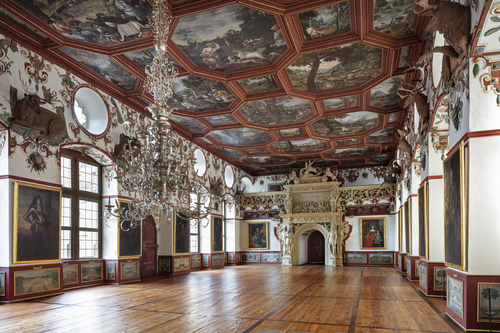
\includegraphics{section_files/figure-pdf/cell-4-output-2.png}

\begin{Shaded}
\begin{Highlighting}[]
\NormalTok{get\_graph()}
\end{Highlighting}
\end{Shaded}

\begin{verbatim}
AttributeError: module 'numpy' has no attribute 'bool8'
---------------------------------------------------------------------------
AttributeError                            Traceback (most recent call last)
Cell In[8], line 1
----> 1 get_graph()

Cell In[5], line 166, in get_graph()
    165 def get_graph():
--> 166     import VizKG.visualize as vkg
    167     results_graph1 = run_query(endpoint_url, query_graph)
    168     #print(results_graph1)
    169     #print('---')

File ~/.python/current/lib/python3.10/site-packages/VizKG/__init__.py:1
----> 1 from .visualize import *

File ~/.python/current/lib/python3.10/site-packages/VizKG/visualize.py:3
      1 import sys
      2 import random
----> 3 from .utils import set_chart, set_dataframe, chartdict
      4 from .charts import Chart
      5 class VizKG:

File ~/.python/current/lib/python3.10/site-packages/VizKG/utils/__init__.py:1
----> 1 from .util import *
      2 from .chartdict import chartdict

File ~/.python/current/lib/python3.10/site-packages/VizKG/utils/util.py:9
      6 from difflib import SequenceMatcher
      7 import ssl
----> 9 from .chartdict import chartdict as chart_dictionary
     11 def set_chart(chart_input):
     12     """
     13     Setter of chart based on chart input
     14 
   (...)
     17     :return: (str) chart: The available chart   
     18     """

File ~/.python/current/lib/python3.10/site-packages/VizKG/utils/chartdict.py:1
----> 1 from VizKG.charts import *
      2 """
      3 Dictionary of visualization charts 
      4 """
      5 chartdict = {
      6     'imagegrid': ImageGrid,
      7     'timeline': Timeline,
   (...)
     29     'radarchart': RadarChart
     30 }

File ~/.python/current/lib/python3.10/site-packages/VizKG/charts/__init__.py:7
      5 from .graph import Graph
      6 from .map import Map
----> 7 from .table import Table
      8 from .imagegrid import ImageGrid
      9 from .dimensions import Dimensions

File ~/.python/current/lib/python3.10/site-packages/VizKG/charts/table.py:2
      1 from .chart import Chart
----> 2 import plotly.figure_factory as ff
      3 from IPython.display import display
      4 import pandas as pd

File ~/.local/lib/python3.10/site-packages/plotly/figure_factory/__init__.py:32
     30 if optional_imports.get_module("pandas") is not None:
     31     from plotly.figure_factory._county_choropleth import create_choropleth
---> 32     from plotly.figure_factory._hexbin_mapbox import create_hexbin_mapbox
     33 else:
     35     def create_choropleth(*args, **kwargs):

File ~/.local/lib/python3.10/site-packages/plotly/figure_factory/_hexbin_mapbox.py:2
      1 from plotly.express._core import build_dataframe
----> 2 from plotly.express._doc import make_docstring
      3 from plotly.express._chart_types import choropleth_mapbox, scatter_mapbox
      4 import numpy as np

File ~/.local/lib/python3.10/site-packages/plotly/express/__init__.py:15
      9 if pd is None:
     10     raise ImportError(
     11         """\
     12 Plotly express requires pandas to be installed."""
     13     )
---> 15 from ._imshow import imshow
     16 from ._chart_types import (  # noqa: F401
     17     scatter,
     18     scatter_3d,
   (...)
     49     density_mapbox,
     50 )
     53 from ._core import (  # noqa: F401
     54     set_mapbox_access_token,
     55     defaults,
     56     get_trendline_results,
     57     NO_COLOR,
     58 )

File ~/.local/lib/python3.10/site-packages/plotly/express/_imshow.py:4
      2 from _plotly_utils.basevalidators import ColorscaleValidator
      3 from ._core import apply_default_cascade, init_figure, configure_animation_controls
----> 4 from .imshow_utils import rescale_intensity, _integer_ranges, _integer_types
      5 import pandas as pd
      6 import numpy as np

File ~/.local/lib/python3.10/site-packages/plotly/express/imshow_utils.py:24
      9 _integer_types = (
     10     np.byte,
     11     np.ubyte,  # 8 bits
   (...)
     19     np.ulonglong,
     20 )  # 64 bits
     21 _integer_ranges = {t: (np.iinfo(t).min, np.iinfo(t).max) for t in _integer_types}
     22 dtype_range = {
     23     np.bool_: (False, True),
---> 24     np.bool8: (False, True),
     25     np.float16: (-1, 1),
     26     np.float32: (-1, 1),
     27     np.float64: (-1, 1),
     28 }
     29 dtype_range.update(_integer_ranges)
     32 DTYPE_RANGE = dtype_range.copy()

File ~/.python/current/lib/python3.10/site-packages/numpy/__init__.py:410, in __getattr__(attr)
    407     import numpy.char as char
    408     return char.chararray
--> 410 raise AttributeError("module {!r} has no attribute "
    411                      "{!r}".format(__name__, attr))

AttributeError: module 'numpy' has no attribute 'bool8'
\end{verbatim}


\backmatter


\end{document}
